\cotefile{22}
\scanpage{2}
C. R. Acad. Sc. Paris, t. 257, p. 2948--2950 (13 novembre 1963). \hfill Groupe 1.

\textsc{Algèbre.} --- \textit{Étude différentielle des anneaux locaux réguliers : applications.}
Note (*) de M. \textsc{Jean-Pierre Jouanolou}, présentée par M. René Garnier.

Le paragraphe 1 donne pour les anneaux locaux usuels (localités, localités analytiques, etc.) une caractérisation différentielle de régularité. Remarquant que, pour ces anneaux, la complétion se fait de façon « séparable », on montre que la réduction et la normalité analytiques en résultent simplement.

1. Les critères différentiels de régularité de Nakai, Suzuki et Mount font \deleted{apparaître}\inserted{appel} en caractéristique $p>0$ \inserted{\unsure{à}}une \deleted{condition}\inserted{\unsure{l'hypothèse}} de réduction analytique (il y a des exemples contraires sinon). L'énoncé suivant permet d'éviter cette condition dans les cas usuels :

\margin{\figure{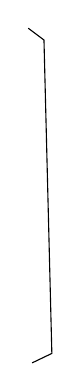
\begin{tikzpicture}[x=1cm,y=1cm]\draw (0.15,0)--(0.4,0.12)--(0.3,4.1)--(0.1,4.25);\end{tikzpicture}}}
\textsc{Proposition 1.} --- \textit{Soient $A$ un anneau local régulier équicaractéristique tel que $D(A)$ soit plat et $\mathfrak{a}$ un idéal de $A$ tel $A/\mathfrak{a}$ soit réduit.}
\margin{\figure{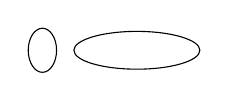
\begin{tikzpicture}\draw (0,0) ellipse (0.18 and 0.28);\draw (1.2,0) ellipse (0.8 and 0.24);\end{tikzpicture}}}

\textit{Les assertions suivantes sont équivalentes :}

\textit{(a) $A/\mathfrak{a}$ est régulier;}

\textit{(b)} $\operatorname{Tor}^{1}_{A/\mathfrak{a}}(A/\mathfrak{m},D(\deleted{A}\inserted{A/\uline{a}}))=0$;

\textit{(c)} $\operatorname{Tor}^{i}_{A/\mathfrak{a}}(A/\mathfrak{m},D(\deleted{A}))=0$ \textit{pour tout $i$ supérieur ou égal à $1$} ($\mathfrak{m}$ \textit{désignant l'idéal maximal de} $A$).

\textit{De plus, si $D(A)$ est libre, (a) équivaut à :}

\textit{(d) $D(A/\mathfrak{a})$ est libre.}

\textsc{Corollaire 1.} --- \textit{Soient $k$ un corps valué complet de caractéristique $p>0$ et tel que $(k:k^p)<+\infty$, $B$ une algèbre de séries convergentes sur $k$ et $A$ un anneau réduit localisé d'un anneau quotient de $B$. Pour que $A$ soit régulier, il faut et il suffit que $D(A)$ soit libre.}

\textsc{Corollaire 2} [Kunz \textsuperscript{(3)}]. --- \textit{Pour qu'une localité \uline{réduite} $A$ soit régulière, il faut et il suffit que son module de différentielles absolu $D(A)$ soit libre.}
\margin{\unsure{contenu dans le critère jacobien} \unsure{---}}

\textsc{Corollaire 3} [Suzuki \textsuperscript{(10)}, Mount \textsuperscript{(5)}]. --- \textit{Soit $A$ un anneau local noethérien analytiquement réduit de caractéristique $p>0$ et tel que le séparé $D'(A)$ \uline{soit de type fini}. Alors, pour que $D'(A)$ soit libre, il faut et il suffit que $A$ soit régulier.}
\margin{\unsure{assez rare !}}

La proposition 1 fournit des critères pour que l'ensemble des points non réguliers du spectre d'un anneau (lieu singulier) soit un fermé, notamment :

\margin{\figure{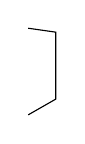
\begin{tikzpicture}\draw (0,1.1)--(0.35,1.05)--(0.35,0.2)--(0,0);\end{tikzpicture}}}
\textsc{Proposition 2.} --- \textit{Si $A$ est un anneau global régulier équicaractéristique tel que $D(A)$ soit libre, le lieu singulier de toute $A$-algèbre affine $B$ est fermé.}
\margin{\unsure{Séries formelles ??}}

En particulier :

\textsc{Proposition 3.} --- \textit{Soit $G$ un schéma en groupes régulier sur un corps parfait. Alors tout schéma de type fini sur $G$ a un lieu singulier fermé.}
\margin{\unsure{Canonique}}

2. Dans tout ce qui suit, $A$ étant un anneau local, nous désignerons par $L_A$ son corps résiduel et par $K_A$ son corps de fractions s'il est intègre.

\mspage{1}
